% !TEX root = ../main_text.tex
% !TeX encoding = UTF-8
\chapter{Introdução} \label{chap:introducao}

   %\todo[inline]{contextualização lógica}
	%intro geralzona
	O recente progresso na obtenção e manipulação de informações, em conjunto com a ascensão da tecnologia da microeletrônica, comunicação e sensores, proporcionou um enorme estímulo no desenvolvimento de sistemas computacionais inteligentes de comunicação e \wearables, todos sendo dispositivos embarcados \citep{Jozwiak2017}.
	%
	O projeto de sistemas computacionais está mais complexo que nunca. A demanda por curto tempo para disponibilidade ao mercado, somado ao fato dos produtos exigirem propriedades de corretude, rapidez, confiabilidade e preço acessível, representam um desafio para projetistas de sistemas embarcados em geral.
	Sistemas computacionais embarcados (também nomeados pela literatura como sistemas embarcados ou sistemas embutidos) possuem muitos componentes implementados tanto em \hs\ e esta decisão de escolha de local de implementação será o tema principal abordado neste documento com foco em dispositivos \wearable.

	% embedded 
   %\todo[inline]{A parte de wearable vc tem q explorar mais no capitulo 1 tb, como construcao da motivacao. Uma introducao tem q ser a sequinte sequencia}
	Os sistemas computacionais embutidos são produtos que utilizam processadores ou controladores e podem estar desde fornos de microondas, até sistemas de controle de aeronaves.
   São computadores situados em dispositivos e que sua presença não é imediatamente óbvia.
	Requerem técnicas na qual difere das utilizadas para \design\ de computadores de propósito geral ou aplicações de \software\ dessas máquinas \citep{Wolf1994}.  
	Em 2015, foi previsto um total de 6,5 bilhões de dispositivos ativamente conectados para o ano de 2016, segundo notícias da empresa de pesquisa e consultoria Gartner \citep{RobvanderMeulen2015}.
	
	% wearable
	No âmbito de sistemas embutidos, existe um subconjunto na qual possui o propósito de integrar-se ao sistema corporal expandindo suas capacidades. 
	Esses dispositivos `vestíveis', chamados de sistemas \wearables, envolvem grande volume de dados de múltiplos sensores ou outros sistemas e são requeridos para prover serviço autônomo, contínuo, em um longo período de tempo.
   Diferentemente de \textit{smartphones} e \textit{tablets}, os \wearables\ são tecnologias eletrônicas ou computadores que são incorporados ao vestuário dos usuários criando uma integração cada vez mais intensa entre tecnologia e ser humano. 
   Sua tendência é superar os dispositivos manuais como computadores e telefones pois são dispositivos mais sofisticados pela existência de recursos sensoreais e escaneamento.
   %
   Cerca de 20\% da população possui pelo menos um dispositivo sendo que 10\% utiliza-o todos os dias \citep{lee2016information}.
   São dispositivos que permitem benefícios como um estilo de vida inspirado em dados \textit{fitness} até realidade aumentada preenchida por objetos virtuais.
	Tais dispositivos demandam de uma alta performance e/ou baixo consumo de energia, sem apresentar \textit{trade-off} de confiabilidade e segurança entre outros. % \citep{Jozwiak2017}.
	%
	Segundo o trabalho de \citet{Jozwiak2017}, com computação de alta performance e estudos em gasto energético eficiente, foi possível a facilitação do rápido progresso da computação móvel e autônoma.
	%Tudo isso deve-se à possibilidade de comunicar-se com a rede global de comunicação, combinada com o progresso de sensores e atuadores, criando novas oportunidades importantes de projeto.
	%%Exemplos disso são indústrias inteligentes, cidades e casas, bem como setores de IoT, sistemas móveis como automóveis inteligentes, computação móvel como \textit{smartphones}, comunicação e, não menos importante, os sistemas computacionais \wearable.
	Sistemas computacionais \wearables\ podem ser definidos como `embutidos que foram inseridos em ambiente \mobile\ de seus usuários, não exercendo a mesma atividade' e seu propósito é criar dispositivos com acesso constante, conveniente, portátil e principalmente \textit{hands-free}, aplicando não só na área de saúde e esportiva, mas também em entretenimento e assim por diante.

   %\todo[inline]{1- Apresnetar o problema:}
   \section{Problema}
	% intro particionamento
	A redução do ciclo de comercialização de um produto e o aumento de sua eficiência de desenvolvimento de projeto tem se tornado uma preocupação na área de \design\ de sistemas embarcados, incluindo também os \wearables.
	E por este motivo, a técnica de particionamento \hs\ tem sido uma das principais tecnologias para o desenvolvimento de sistemas embarcados em geral, desde que, este afeta a performance do sistema como um todo. 
   Para \citet{Hassine2017}, uma das soluções mais elegantes na computação que provê otimizações sistêmicas sobre essas circunstâncias é por meio do particionamento \hs.
	Segundo \citet{Wolf1994}, sistemas embutidos gerais são considerados únicos pelo fato da necessidade de um \codesign\ de \hs. 
   As pesquisas em \codesign\ de \hs\ têm como objetivo o \design\ de sistemas heterogêneos, visando performance, custo e metas de confiabilidade \citet{Edwards1994}.
	
   \begin{comment}
   
   Um exemplo simbólico de \codesign\ para o particionamento pode ser ilustrado na Figura \ref{fig:rt-edwards_partitioning} no qual um módulo em \software\ é substituído por um componente em \hardware\ executando a mesma tarefa mas com maior performance.
   
   \begin{figure}[h] \centering
   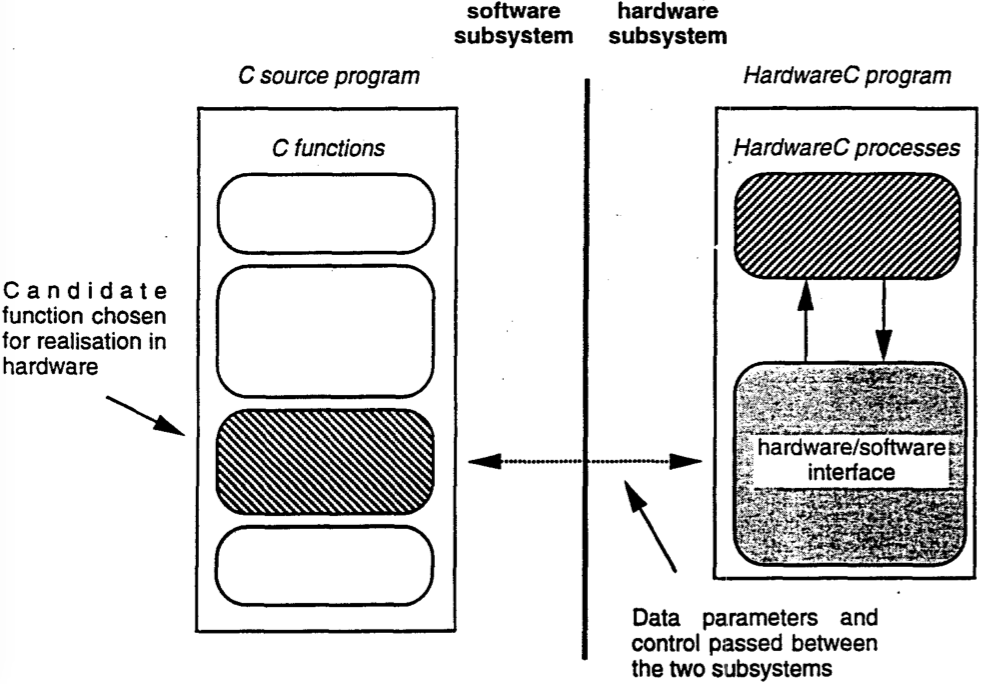
\includegraphics[width=0.7\textwidth]{img/rt-edwards_partitioning.png}
   \caption{Ilustração de um particionamento no \codesign\ de um sistema embarcado. Fonte: \citet{Edwards1994}.}
   \label{fig:rt-edwards_partitioning}
   \end{figure}
\end{comment}

	\citet{Hidalgo1997} dizem que o objetivo principal é o balanceamento de todas as tarefas de forma a otimizar alguns objetivos de sistema sobre determinadas restrições.
	Agrupar específicos conjuntos de instruções de uma aplicação e então mapear esses grupos tanto em \hs.
	%Os grupos designados ao \software\ são executados sequencialmente pelo respectivo processador do sistema enquanto os mapeados em \hardware\ são implementados por uma combinação customizada ou por circuitos sequenciais \citep{Sass2010}.

	% particionamento
	%Quando necessita de performance ao realizar o \codesign\ (termo referente ao inglês \textit{Participatory Design}) de \hs\ para sistemas embutidos, o problema de qual função do sistema deverá ser implementada em \hardware\ ou em \software\ emerge e esse problema é conhecido por particionamento \hs\ (\textit{hardware/software partitioning}).
	%Um significante esforço foi posto nesta área nos últimos dez anos, segundo \citet{Trindade2016}.
   
   Um desafio de \design\ é combinar a flexibilidade de demanda pelos vários ambientes e aplicações, e a alta performance exigida em tarefas com o baixo consumo de energia requerido para maximizar o tempo de uso da bateria.

   %\todo[inline]{3- Motivacao pra resolver este problema:}

	%Com o desenvolvimento de sistemas embutidos cada vez mais complexos, o particionamento \hs\ tornou-se um problema de otimização em \codesign\ de sistemas \citep{Yan2017}. 
   A motivação é que, tal problema que envolve \design\ colaborativo e multidisciplinar, é um passo-chave no \design\ de produtos modernos \citep{Trappey2016}. 
   Implementações que baseiam-se somente em módulos de \software\ possuem mais flexibilidade e menos custosos, entretanto, seu custo eleva-se em termos de tempo de execução. Uma implementação de \hardware\ customizada de um conjunto de computações proverá uma eficiência energética e \speedup\ maior relativa à implementações em \software\ \citep{Zhang2008, Hassine2017, Wolf1994, Canis2011, Stone2010}.

   % combinação de fpga com cpu
   A tendência hoje para \design\ é na combinação das funções do processador com os recursos dos arranjo de portas programáveis em campo (FPGAs, do inglês \textit{Field-Programmable Gates Array}) formando um sistema computacional híbrido. %, exemplo exibido na Figura \ref{fig:i-soc}. %\citep{Plessl2003}
   %O conceito de CSoC é importante quando necessita da construção de sistemas computacionais que podem utilizar de circuitos junto à um processador como é o caso de sistemas embutidos.
	Ao utilizar do FPGA para o problema de particionamento, é possível acelerar uma aplicação usando recursos de \hardware\ melhorando no desempenho e eficiência energética em comparação com o \software\ executado inteiramente em um processador \citep{Cong2009, Lo2009, Zhang2008a}. 
   %A Microsoft em \citeyear{Putnam2014} aceleraram o \textit{Bing Search} em duas vezes com a utilização de FPGAs em seus \textit{data centers} \citep{Putnam2014}.
   %além da aquisição da Altera, uma das duas maiores vendedoras de FPGAS no mundo, pela Intel em \citeyear{Maan2015} por cerca de $ 16.7 $ bilhões de dólares \citep{Maan2015}.


   %{4- Contribuicao ao resolver o problema:}

   %{5- Objetivos:}
   
   Este trabalho então, propõe o estudo e aplicação de técnicas de particionamento dentro do conjunto de aplicações e sistemas \wearable, na qual, possui restrições significativas como bateria, recursos e custo.

\section{Objetivos da Dissertação}
	Este trabalho tem como objetivo a abordagem do particionamento \hs\ bem como sua importância no mundo de sistemas computacionais embutidos, com foco em sistemas \wearables\ apresentando algumas soluções utilizadas atualmente.

    \begin{itemize}
      %\item Apresentação do tema de projeto de sistemas computacionais \wearable\ por meio do particionamento \hs;
      %\item Apresentação de uma abordagem metodológica criada para o uso ao problema aplicado no contexto desses sistemas \wearable, na qual possuem restrições relacionados ao custo energético e recursos.
      
         \item Introdução de sistemas computacionais \wearables\ e apresentação do problema de particionamento \hs\ no âmbito de de sistemas computacionais embutidos, com foco em sistemas \wearables;
         
         \item Apresentação das principais soluções apresentadas ao logo dos anos e as utilizadas atualmente, bem como as ferramentas HLS como LegUp e OpenCL para a geração de sistemas computacionais que usufruem de aceleradores em \hardware.
         
         \item Exposição da abordagem metodológica a ser utilizada para a procura da solução do problema de particionamento \hs\ apresentado.
    \end{itemize}

   \subsection{Justificativa}

   %{2- Justificativa pq eh um problema relevante:}
	A justificativa para a realização deste é que, além do tema de particionamento ser proposto recentemente, com o desenvolvimento de \designs\ mais complexos, esse problema de decisão torna-se cada vez mais desafiador para os \designers\ de projeto, no qual o grande requisito para eficiência necessariamente segue junto com a alta velocidade de processamento \citep{Trindade2016, Arato2005, Yan2017}.
	
	Dessa forma, pesquisá-lo com foco em sistemas \wearable\ torna-o ainda mais necessário pela pouca atenção dada pelo meio científico até o presente momento, como será demonstrado no decorrer do documento, principalmente pelo ampla utilização que este tipo de produto vem ganhando no espaço comercial.


   \subsection{Contribuição}
    
      O trabalho consiste numa busca sobre o aprimoramento de performance de um dispositivo computacional \wearable\ visando os respectivos gastos relativos ao uso de aceleradores em \hardware\ como recursos, gasto energético, área utilizada e outros itens que serão discutidos neste documento. 
       

\section{Organização da Dissertação}
	Os demais capítulos deste trabalho estão organizados da seguinte forma: 
   No Capítulo \ref{chap:revisao_bibliografica} é apresentada uma revisão bibliográfica do problema, abordando alguns métodos de fundamental importância para este trabalho. 
   No Capítulo \ref{chap:relacionados} são descritos alguns trabalhos relacionados ao tema abordado. 
   Nos Capítulos \ref{chap:design} e \ref{chap:met2} são apresentadas as metodologias, sendo a primeira a exibição do processo de \design\ e a segunda a metodologia proposta. 
   %No Capítulo \ref{chap:experimentos} \todo{são?} apresentados os resultados e suas considerações para o problema. 
   No Capítulo \ref{chap:conclusao} são apresentadas as conclusões parciais e propostas de trabalhos futuros.